\documentclass{article}

\usepackage[utf8]{inputenc}
\usepackage{hyperref}
\usepackage{amssymb}
\usepackage{amsmath}
\usepackage{polski}
\usepackage{a4wide}
\usepackage{graphicx}

\author{Krzysztof Chrobak}
\title{Sieci Neuronowe \\ \small{Bayesian Hierarchical Community Discovery}}

\begin{document}

\maketitle

\begin{abstract}
W związku z wzrastającą popularnością portali społecznościowych konieczne stało
się rozwinięcie metod automatycznego przetwarzania grafów znajomości. Jednym z
praktycznych problemów tej dziedziny jest segmentacja struktury powiązań na
kręgi zawierające osoby mające ze sobą coś wspólnego. Projekt zawiera implementację
metody znajdowania hierarchicznej struktury grup znajomych z \cite{BHCD}.
\end{abstract}

\section{Implementacja algorytmu}
\subsection{Usprawnienia}
Ponieważ praca \cite{BHCD} podaje jedynie pseudokod algorytmu, konieczne
okazało się opracowanie kilku usprawnień umożliwiających zastosowanie metody do
większych grafów.

\subsubsection{Kolejka priorytetowa}
Kolejka priorytetowa zawierająca możliwe operacje połączenia drzew zaimplementowana
naiwnie szybko rośnie do astronomicznych rozmiarów. Wiemy, że część ze znajdujących
się w niej operacji nie będzie dało się już wykonać, więc rozwiązaniem tego
problemu jest okresowe filtrowanie jej zawartości. Jeśli takie filtrowanie
przeprowadzamy tylko wtedy, kiedy mamy pewność że pozbędziemy się ponad połowy
elementów, to zamortyzowany koszt tej operacji jest stały.

\subsubsection{Krawędzie w grafie}
Pseudokod algorytmu sugeruje tworzenie potencjalnych połączeń pomiędzy wszystkimi 
drzewami w lesie. W mojej implementacji ograniczyłem się do połączeń pomiędzy
drzewami, między którymi istnieją krawędzie w grafie znajomości, co bardzo pomaga
gdy mamy do czynienia z grafem rzadkim (np. dane NIPS opisane niżej)

\subsubsection{Funkcje $\Gamma$ i $B$}
Stablicowanie wartości funkcji $\Gamma$ znacznie przyspieszyło działanie algorytmu,
ponieważ najczęściej wywoływaną funkcją w całym programie jest obliczanie funkcji
$B(a, b) = \frac{\Gamma(a)\Gamma(b)}{\Gamma(a+b)}$.

\subsection{Złożoność}
Opisane powyżej usprawnienia mają wpływ tylko na stałą, natomiast teoretyczna
złożoność pozostaje taka sama jak w pracy: $O(n^2\log n)$, gdzie $n$ jest
liczbą wierzchołków grafu. Usprawnienie polegające na rozważaniu połączeń tylko
tych drzew, między którymi istnieją krawędzie w grafie znajomości niestety nie
zmienia tego stanu rzeczy. Dla każdego $n$ istnieje nawet graf o stopniu
wierzchołka co najwyżej 2 i taka kolejność łączeń, dla której algorytm wykona
$\Omega(n^2\log n)$ operacji.

\subsection{Technologie}
Ponieważ większość obliczeń w algorytmie nie daje się wyrazić jako operacje na 
macierzach, efektywna implementacja musiała zostać zrealizowana w języku 
niskiego poziomu. Ze względu na dostępność świetnych narzędzi do debugowania i
profilowania algorytm zaimplementowałem w C++. 

Skrypty przetwarzające zbiory danych, generujące wykresy i oceniające jakość 
wyjścia napisałem w Pythone.


\section{Eksperymenty}
\subsection{Klasztor}
W pracy \cite{BHCD} autorzy sprawdzili jakość wyników na danych pochodzących 
z obserwacji 18 mnichów w klasztorze. Rysunek \ref{sampson} przedstawia ilość
pozytywnych (present) i negatywnych (absent) relacji pomiędzy poszczególnymi 
mnichami. Otrzymane drzewo znajomości znajduje się w załączonym pliku sampson.pdf,
ponieważ jego format uniemożliwił wstawienie go do raportu.

\begin{figure}
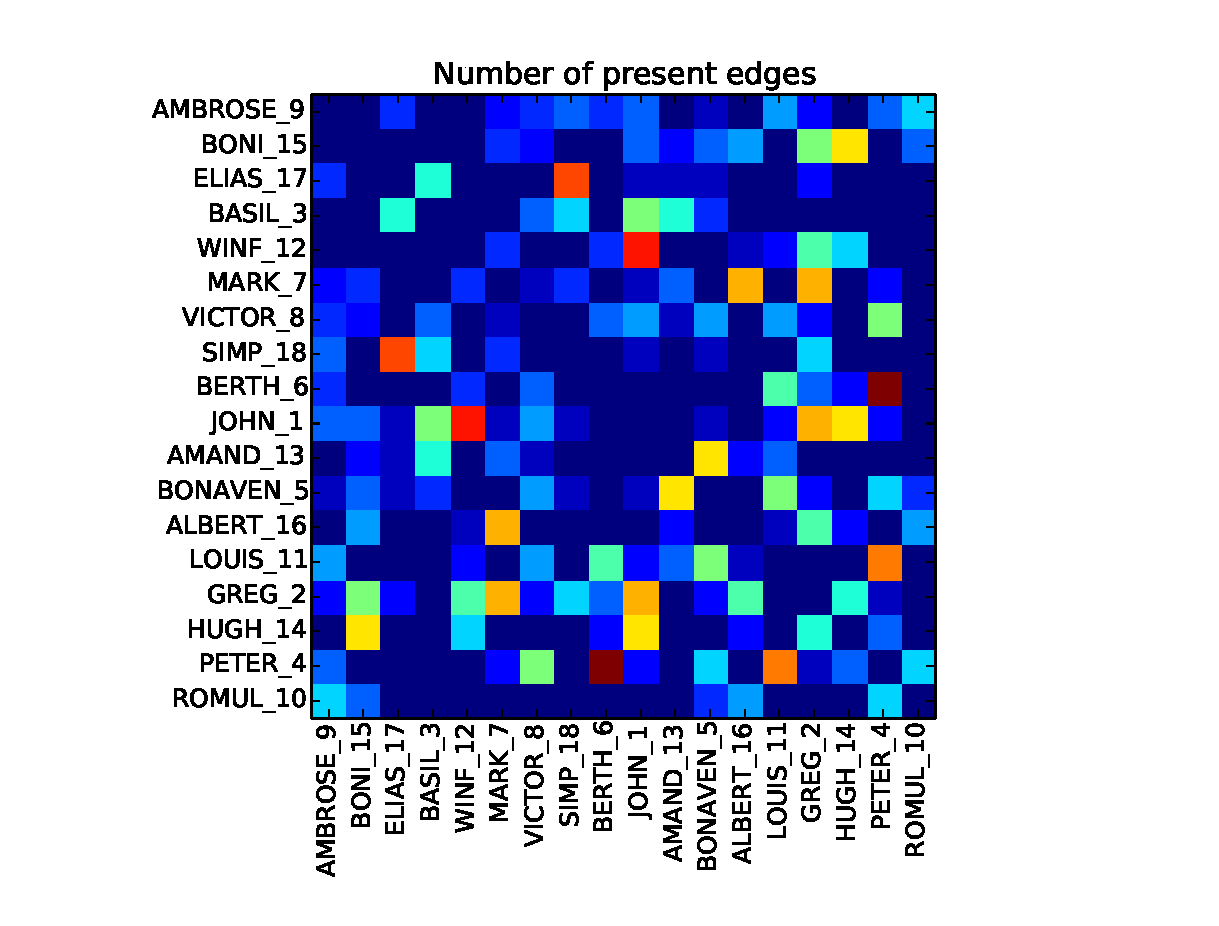
\includegraphics[width=0.5\textwidth]{sampson_present.pdf}
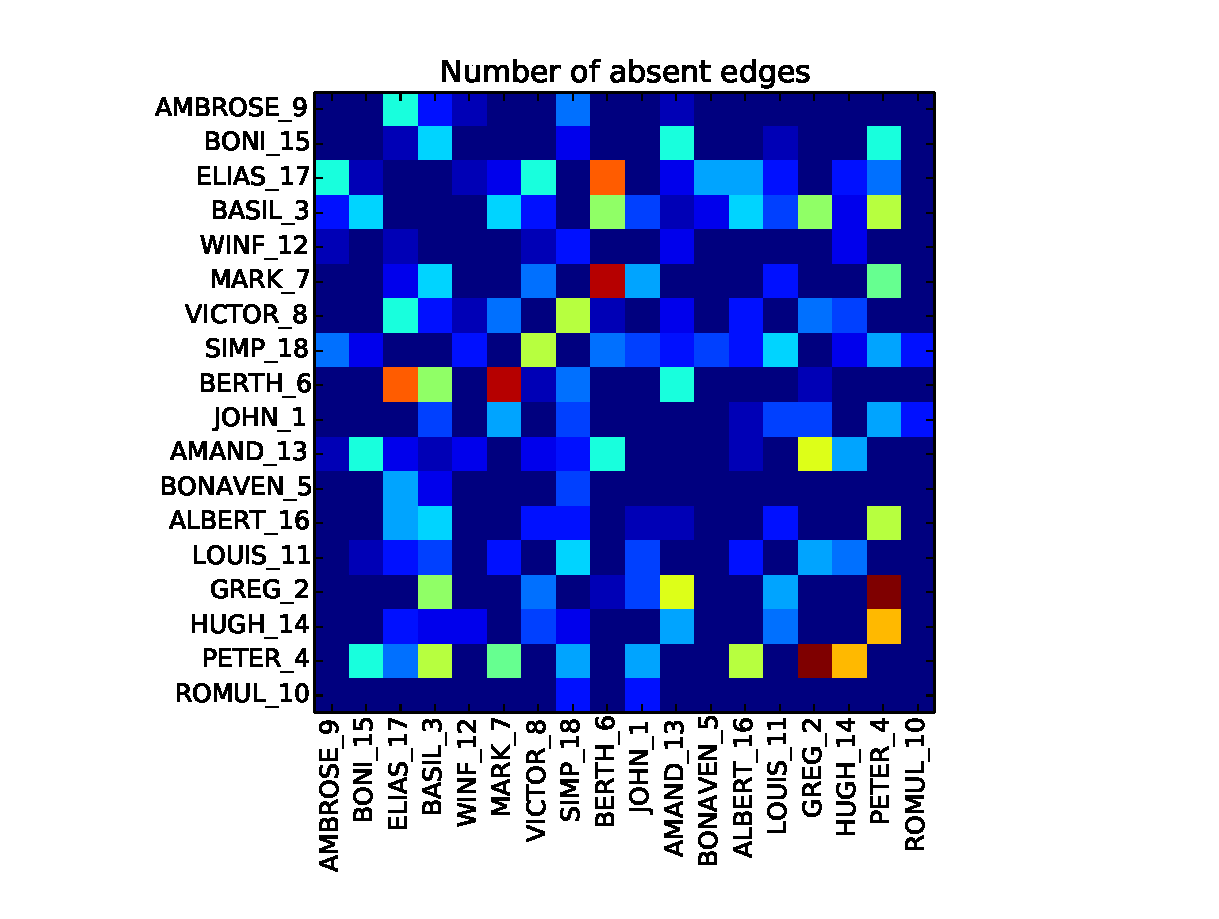
\includegraphics[width=0.5\textwidth]{sampson_absent.pdf}
\caption{Relacje w klasztorze}
\label{sampson}
\end{figure}

\subsection{Repozytoria}
Zaczynając pracę nad projektem planowałem przetestować algorytm na repozytoriach
git-a z kodem kernela i nodejs, ale po wyekstrahowaniu grafu "znajomości" okazało
się, że w danych nie ma oczywistej struktury zawierającej sensowne klastry. Znalazło
to odzwierciedlenie w wynikach, ponieważ algorytm umieszczał wszystkich autorów
commitów w jednej składowej.

Przyjąłem, że między wybranymi autorami jest tyle pozytywnych krawędzi, ile jest
plików w których obaj wprowadzili zmiany.

\subsection{NIPS}
Jakość znajdowanych kręgów sprawdziłem na zbiorze danych pochodzących z
konferencji NIPS. Wierzchołki w grafie to autorzy, a ilość krawędzi pomiędzy
dwoma autorami odpowiada ilości wspólnych publikacji. Za miarę jakości
przyjąłem poniższą funkcję ($G$ - graf, $\delta(G')$ - ilość krawędzi wewnątrz
$G' \subseteq G$, $\phi(G')$ - ilość krawędzi wychodzących z $G' \subseteq G$):
$$q(G') = \frac{\delta(G')}{\phi(G') + \delta(G')}$$
Wystarczyło liczyć tylko pozytywne krawędzie, bo w tym zbiorze danych nie
występują negatywne relacje (odpowiadałyby np. negatywnej recenzji).

Rysunek \ref{cdf} przedstawia empiryczne dystrybuanty jakości kręgów
znalezionych przez algorytm (inferred) i tych obecnych w danych (given).
Kręgiem obecnym w danych jest pojedyncza publikacja, natomiast w drzewie
zwróconym przez algorytm za krąg uznajemy każde poddrzewo $T$, takie że
$|v(T)| \in [2, 200]$.

\begin{figure}
\begin{center}
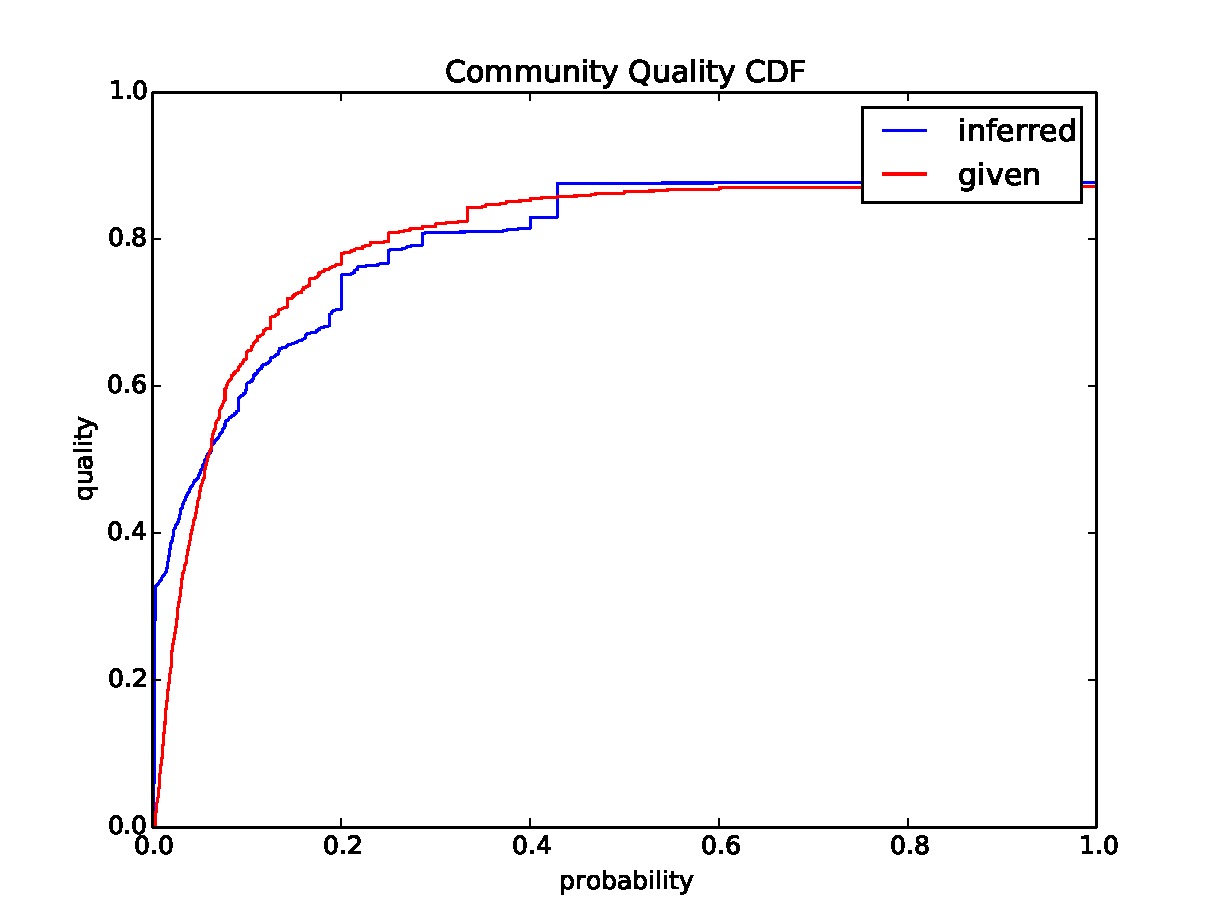
\includegraphics[width=0.7\textwidth]{quality_cdf.pdf}
\end{center}
\caption{Empiryczna dystrybuanta jakości znalezionych kręgów}
\label{cdf}
\end{figure}

\begin{thebibliography}{4}
\bibitem{BHCD}
    \href{http://papers.nips.cc/paper/5048-bayesian-hierarchical-community-discovery.pdf}
    {Bayesian Hierarchical Community Discovery}\\
    Blundell, Charles and Teh, Yee Whye\\
    Advances in Neural Information Processing Systems 26
\end{thebibliography}

\end{document}
